\section{Tensorflow CNN}

Δημιουργήθηκαν δύο δίκτυα με την βοήθεια της tensorflow. Και τα δύο έχουν κοινή αρχιτεκτονική , αλλα διαφορετικούς optimizer.
Η αρχιτεκτονική τους απεικονίζεται στην εικόνα \ref{f:g9}. Στο 1ο δίκτυο χρησιμοποιήθηκε ο στοχαστικός optimizer με ίδιες παραμέτρους με του τελικού from scratch δικτύου (tensorflow CNN-SGD), ενώ στο 2ο χρησιμοποιήθηκε μονο learning rate με τίμη 10e-5 (tensorflow CNN-lr).


\begin{figure}[ht]
	\centering
	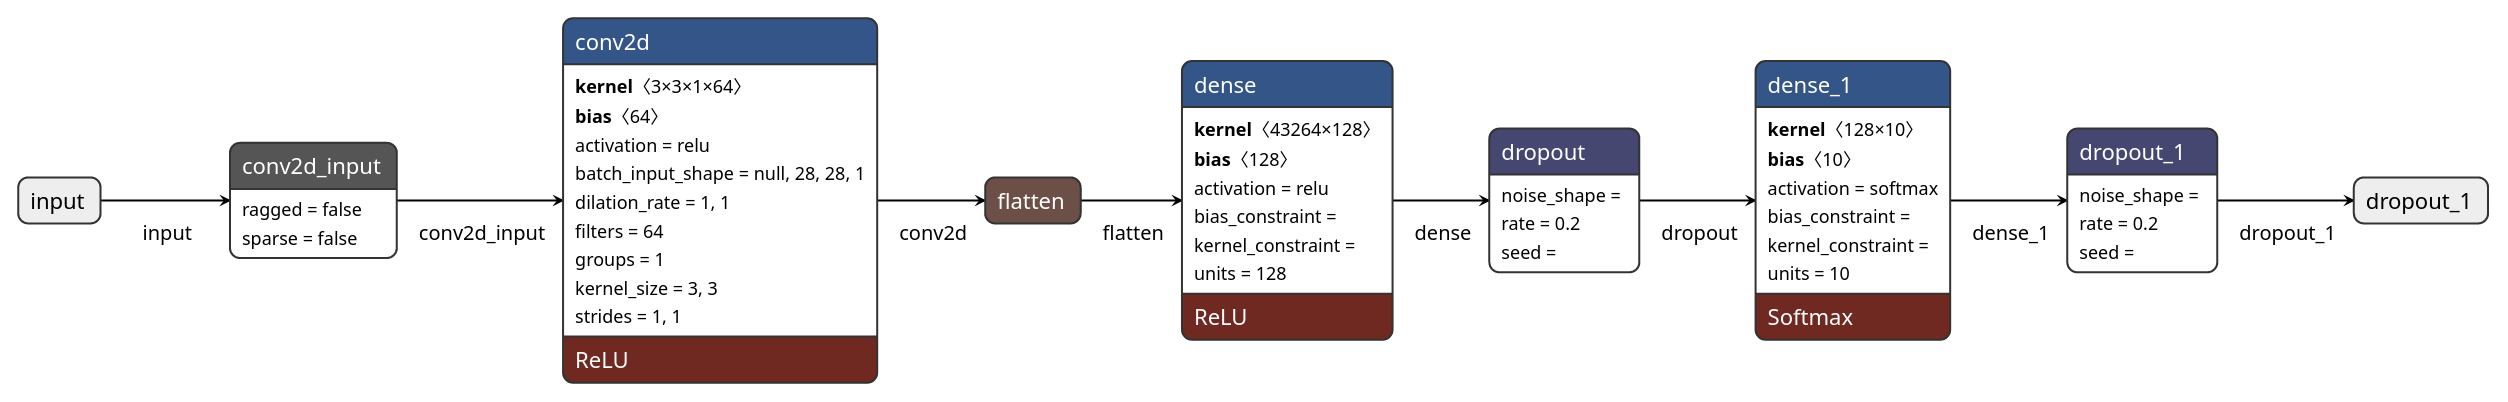
\includegraphics[width=1\linewidth]{Results/tensor.h5.png}
	\caption{ Απεικόνιση αρχιτεκτονική CNN δικτύου}
	\label{f:g9}	
\end{figure}
\clearpage

\section{Numpy CNN vs Tensorflow CNN}

Στο τελευταίο μέρος της εργασίας συγκρίθηκαν τα αποτελέσματα επιτυχίας τόσο στο training οσο και στο testing(validation) μεταξύ του τελικού μοντέλου CNN γραμμένο σε numpy και των δύο μοντέλων CNN γραμμένων σε tensorflow. Το dataset που επιλέχθηκε είναι το ίδιο με πριν, απλά απο 20000 δεδομένα αυξήθηκε σε 40000 δεδομένα στο training και το validation παρέμεινε στο μεγιστο των 10000 δεδομένων.

\subsection{Numpy CNN vs Tensorflow CNN-SGD}

Αρχικά θα συγκρίνουμε το τελικό μοντέλο της numpy και το μοντέλο της tensorflow που έχουν ακριβως την ίδια αρχιτεκτονική (με ίδεις παραμέτρους στον optimizer SGD). Στο διάγραμμα \ref{f:g10} παρατηρούμε τα ίδια αποτελέσματα με τις περιπτώσεις των optimizer στο κεφάλαιο 1,δηλαδή αυξάνεται το accuracy αρκετά γρήγορα και μετά το 80$\%$ παραμένει σχεδόν σταθερό. Απο την άλλη στο διάγραμμα \ref{f:g11} , το validation accuracy ανεβαίνε σχεδόν στο 91$\%$, αλλά το training accuracy δεν μπορεί να ξεπεράσει το 70$\%$. Το κενό μεταξύ των δυο ποσοστών επιτυχίας, υποδηλώνει ότι έχουμε μικρό evaluation bias δηλαδή το dataset που κανουμε validate είναι πολυ μικρό Ίσως αν είχαμε μεγαλύτερο dataset για validation, το μοντέλο να μην έφτανε σε underfitting.

\begin{figure}[ht]
	\centering
	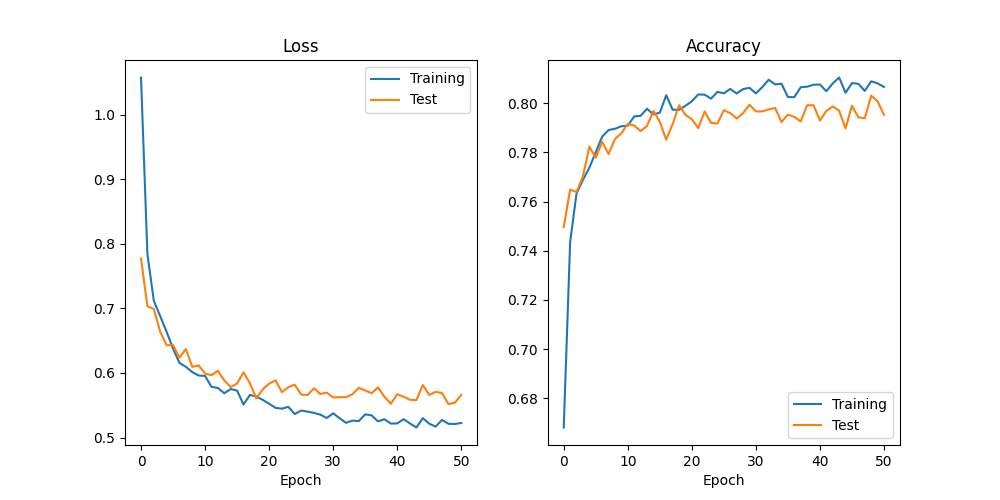
\includegraphics[width=1\linewidth]{Results/40k_withoutdropout_conv_lr.png}
	\caption{ Διάγραμμα loss, accuracy numpy CNN δικτύου}
	\label{f:g10}	
\end{figure}



\begin{figure}[ht]
	\centering
	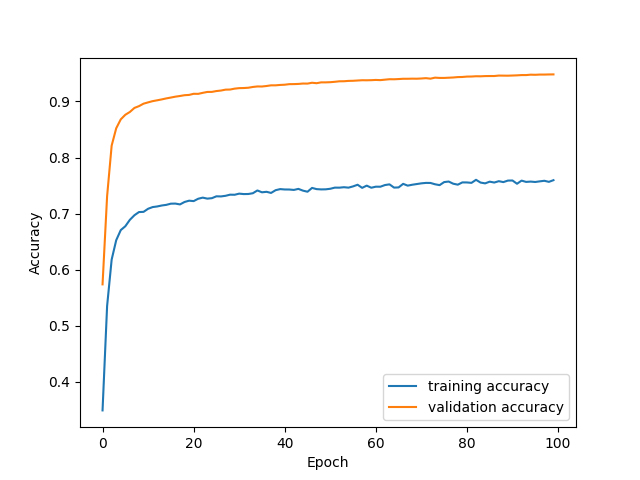
\includegraphics[width=1\linewidth]{Results/tensorflow_lr_moment_decay.png}
	\caption{ Διάγραμμα accuracy tensorflow CNN-SGD δικτύου}
	\label{f:g11}	
\end{figure}
\clearpage

\subsection{Numpy CNN vs Tensorflow CNN-lr}


Στην συνέχεια συγκρίνουμε το τελικό μοντέλο της που δημιουργήθηκε με την βοήθεια της numpy και το μοντέλο της tensorflow παρόμοια αρχιτεκτονική με το 1ο απλά η μόνη παράμετρος που χρησιμοποιείται είναι το learning rate. Στο διάγραμμα \ref{f:g13}
παρατηρόυμε μία πιο ομαλή αυξηση του ποσοστού επιτυχίας απο το προηγούμενο μοντέλο με tensorflow, παρόλα αυτα τα αποτελέσματα παραμένουν τα ίδια, δηλαδή και έδω βλέπουμε underfitting, που ίσως να οφείλεται σε αυτο που αναλύθηκε παραπάνω.

\begin{figure}[ht]
	\centering
	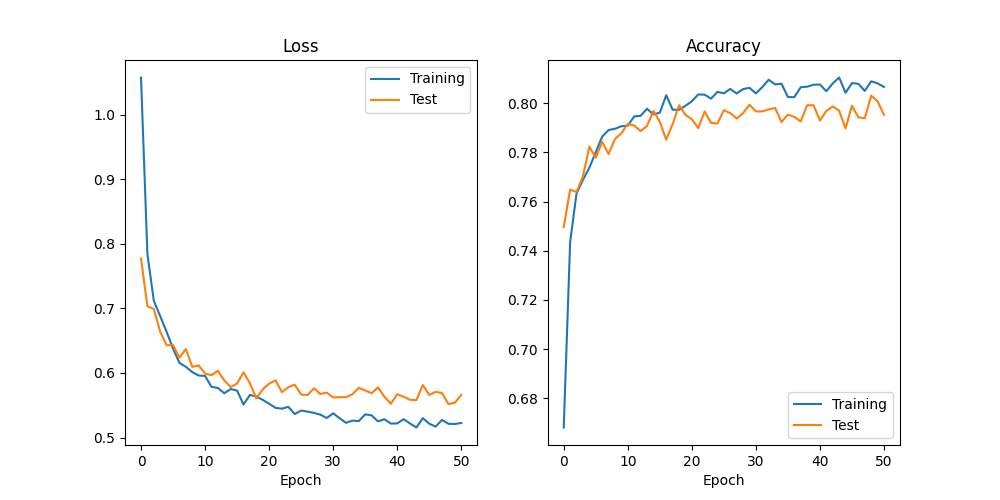
\includegraphics[width=1\linewidth]{Results/40k_withoutdropout_conv_lr.png}
	\caption{ Διάγραμμα loss, accuracy numpy CNN δικτύου}
	\label{f:g12}	
\end{figure}


\begin{figure}[ht]
	\centering
	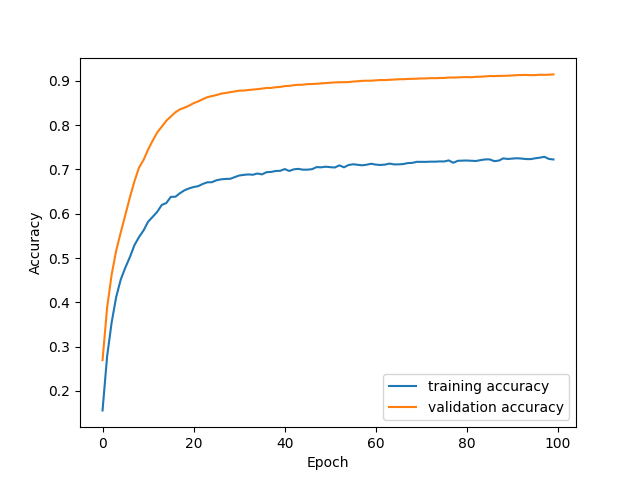
\includegraphics[width=1\linewidth]{Results/tensorflow_lr.png}
	\caption{ Διάγραμμα accuracy tensorflow CNN-lr δικτύου}
	\label{f:g13}	
\end{figure}
\clearpage

\section{Conclusion}
Παρόλο που πέτυχαν ποσοστό επιτυχίας άνω του 90$\%$ έστω και στο validation, τα δύο μοντέλα της tensorflow, το μοντέλο που πραγματοποιήθηκε απο την αρχή μόνο με numpy είχε πιο σταθερά αποτελέσματα, άν και χαμηλά για το συγκεκριμένο dataset. Επισης αξιοσημείωτο είναι το γεγονός ότι ο χρόνος που πήρε τα δύο μοντέλα να επαιδευτουν ήταν περίπου 1 ώρα ένω το from-scratch μοντέλο έκανε περίπου 60 ώρες στον Αριστοτέλη(την συστοιχία του ΑΠΘ). 
